\chapter{Introduction}

%takes p.78~ of ETD Style Manual

This style manual was created to outline the parameters set by necessity to standardize publications produced by graduate students at the University of Oregon. The UO \emph{Style and Policy Manual for Theses and Dissertations} is to be used as a guide to help you establish the physical format and appearance of your thesis or dissertation. However, it does not contain information on all the style issues involved in creating a scholarly work. Some aspects of style (e.g., footnote format and placement, citations and references, tables, and figures) are discipline specific and should be determined in consultation with your advisor and committee.

\section{Style Manuals}

Other manuals~\cite{Codishetal2000} are available in the UO Libraries~\cite{Meyer2000} and the University Bookstore. (See Chapter VII for a list.) Because the student must make a choice concerning style of the manuscript at an early stage, we suggest perusing several different style manuals in the library~\cite{Huetal2000} and consulting with your committee before deciding which style manual to follow. Various disciplines traditionally use a specific style manual~\cite{Conway2000}.

\subsection{Chicago Style Manuals}

Two manuals available from the University of Chicago provide information on most aspects of writing and producing a scholarly work.

\subsubsection{Turabian}

A Manual for Writers of Term Papers, Theses, and Dissertations \footnote{Kate L. Turabian, \emph{A Manual for Writers of Term Papers, Theses, and Dissertations}, 6th ed. (Chicago: University of Chicago Press, 1996).} by Kate L. Turabian is an excellent resource for the graduate student writing a thesis or dissertation. It specifically addresses the mechanics of writing, the presentation of tables and figures, and the major styles of reference documentation. The chapter comparing the two main documentation systems (humanities versus author-date) is particularly useful.

\subsubsection{The Chicago Manual of Style}

\emph{The Chicago Manual of Style}\footnote{The Chicago Manual of Style, The Essential Guide for Writers, Editors and Publishers,
14th ed. (Chicago: University of Chicago Press, 1993).
} provides a thorough explanation of the editing and proofreading issues faced by writers, editors, and publishers. It contains an excellent section on documentation but is very general in scope and must be adapted by the student to meet the style requirements called for in a scholarly thesis or dissertation.The Chicago Manual of Style2 provides a thorough explanation of the editing and proofreading issues faced by writers, editors, and publishers. It contains an excellent section on documentation but is very general in scope and must be adapted by the student to meet the style requirements called for in a scholarly thesis or dissertation.

\section{Some Elements of a Thesis or Dissertation}

\subsection{Headings}

The UO style stipulates that each chapter must begin with the chapter designation
(with a Roman numeral) and the title, both in ALL CAPS, centered, double spaced, 1 inch from the top of the paper. The first page of Chapter I is numbered as page 1. Headings are usually referred to numerically by their level in the hierarchy of organization. The no. 1 head is always the chapter title (ALL CAPS, centered, bold or not). The subsequent levels of headings (no. 2 through as many as necessary) within each chapter can be styled in a variety of ways (any combination of sentence case, small caps, cap and lowercase, bold, underlined, italic, centered, flush left, or run into text) as long as there is some hierarchical logic to the order. If you are using numbered headings, no variation in style is necessary; the numbering system indicates the hierarchy.

The headings in all chapters must be consistent in style. When using nonnumbered heads, you should base your style decisions on the chapter that has the most levels of headings. For example, if Chapter III has four levels of head and the other chapters have only two levels, decide on an appropriate hierarchy for four levels. Use head nos. 1 through 4 in Chapter III and head nos. 1 and 2 in all the other chapters.

Tables are an important part of many dissertations. Table~\ref{LRTtable} is an example of a short data table that might appear in the Materials and Methods or Results section of dissertation or thesis. Note that the title is at the top of the table (not included in it), and the footnotes are explained below the table, not at the bottom of the page. Remember to leave enough space around the table so the title and footnotes do not become confused with the rest of the text. The use of bold or underlining in the table body is discouraged unless needed to highlight an important aspect. All tables must be cited before they appear in the text. Tables most often should be placed at the end of the paragraph in which they are cited (not in the middle of the paragraph). However, they can be placed on the next page to prevent the table from splitting across two pages.

Occasionally, a table contains data that would be presented best in landscape orientation (Table 1.3). Such a table should appear on its own page. These tables can be formatted after separating them from the text with Section Breaks before and after, which will allow the text to be rotated. Sometimes, it is easier to create this table as a separate file and then merge the two pdf files into a single file for uploading.

\begin{table}
\caption{Type 1 error rate of the LRT using the χ2 approximation. Shown are the proportion of 2000 data sets simulated under H0.\label{LRTtable}}
\begin{tabular}{l r r}
\hline
Data set & $\alpha$=0.05 & $\alpha$= 0.01 \\
\hline
Sequence divergence \\
0.05 & 0.068** & 0.020** \\
0.20 & 0.087** & 0.020** \\
0.80 & 0.089** & 0.027** \\
Species number \\
6 & 0.067** & 0.014ns \\
12 & 0.087** & 0.021** \\
18 & 0.112** & 0.034** \\
\hline
**Significance level of 0.005. \\
ns, not significant. 
\end{tabular}
\end{table}

\subsection{Figures}

Any kind of illustrative material that is not a table usually is considered a figure, including such items as maps, photographs, and graphs. Every figure must have a numbered caption, and each category must have its own list of captions in the preliminary pages: List of Tables, List of Figures, etc. Figure~\ref{samplefigure} is a sample of a figure embedded in the text.

If a figure takes up less than half the width of the text area of the page, then it is permissible to place the caption to the right or left of the figure. Otherwise, center the figure between the left and right margins, with the caption below. Figures must take up no more than one complete page. If a figure is larger than one page, experiment with changing the orientation (from Portrait to Landscape), photoreduction, or breaking the figure into multiple figures. For figures that take up the entire text area of the page with no room for the caption, the caption must go on the next page. This situation should be avoided if possible by breaking the figure into separate smaller figures.

Figures must be legible and of “professional” quality. The printing must be clear, with high contrast, and parts must be large enough to be legible after the document is microfilmed. For most figures, any included text should be no smaller than 7 pt. All tables, figures, quotes, appendices, etc., must fit within the designated margins.

\begin{figure}
\centering
	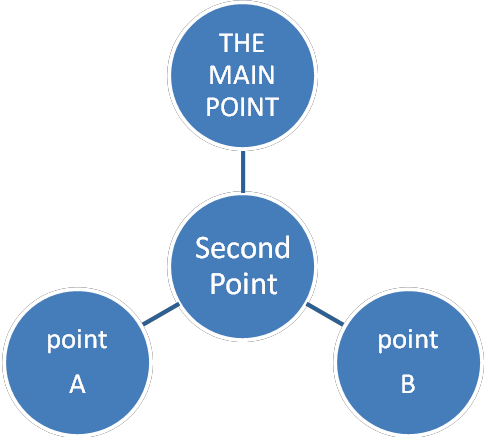
\includegraphics{samplefigure1.png} 
\caption{An example of a centered figure in color. Figure captions usually appear below the figure.\label{samplefigure}}	
\end{figure}